\section{高级实践与未来演进}
本书的重点是可扩展的并行编程。 CUDA C 和 GPU 硬件在我们的示例和练习中主要扮演了编程平台的角色。 
然而,在CUDA C基础上学习的并行编程概念和技能可以很容易地适用于其他并行编程平台。 
例如,正如我们在第 20 章“异构计算集群编程”、“异构计算集群编程:CUDA 流简介”中看到的,
消息传递接口 (MPI) 的大多数关键概念(例如进程、等级和屏障)都有对应的概念。
此外,正如我们在第 20 章“异构计算集群编程”中讨论的那样,支持 CUDA 的 GPU 已在高性能计算 (HPC) 系统中广泛使用。 
对于许多读者来说,CUDA C 可能是一个重要的应用程序开发和部署平台,而不仅仅是一个学习工具。 
因此,读者理解这些应用级别的高级CUDA C特性和实践是很重要的。 
例如,正如我们在第 20 章“异构计算集群编程”中看到的,CUDA 流使 MPI HPC 应用程序能够与计算重叠通信。 
这种能力对于实现整个应用程序的性能目标尤其重要。 
考虑到这一点,本章将为读者概述 CUDA C 和 GPU 计算硬件的高级功能,这些功能对于在应用程序中实现高性能和可维护性非常重要。 
对于每个功能,我们将介绍基本概念以及其在不同代 GPU 计算中的演变简史。 
充分理解这些概念和演变历史将有助于消除对这些功能的一些常见困惑。 目标是帮助读者建立一个概念框架,以便更详细地研究这些功能。

\subsection{主机/设备交互模型}
到目前为止,我们假设了异构计算系统中主机和设备之间的交互的相当简单的模型。 
在这个简单的模型中,如第 2 章“异构数据并行计算”中所述,每个设备都有一个与主机内存或系统内存分开的设备内存(CUDA 全局内存)。 
设备上运行的内核要处理的数据需要通过调用 cudaMemcpy() 函数从主机内存传输到设备内存。 
设备产生的数据还需要通过调用 cudaMemcpy() 函数从设备内存传输到主机,然后才能被主机使用。 
虽然该模型简单且易于理解,但它在应用层面带来了一些问题。

首先,磁盘控制器和网络接口卡等 I/O 设备被设计为在主机内存上高效运行。 
由于设备存储器与主机存储器是分开的,因此输入数据需要从主机存储器传输到设备存储器,
并且输出数据需要从设备存储器传输到主机存储器以在I/O操作中使用。 这种额外的传输会增加 I/O 延迟并降低可实现的 I/O 吞吐量。 
对于许多应用程序来说,I/O 设备直接在设备内存上操作的能力将提高整体应用程序性能并简化应用程序代码。

其次,主机存储器是传统编程系统放置其应用程序数据结构的地方。 有些数据结构很大。 
与主机内存相比,早期支持 CUDA 的 GPU 中的设备内存较小,这迫使应用程序开发人员将大型数据结构划分为适合设备内存的块。 
例如,在第 18 章“静电势图”中,三维 (3D) 静电能量网格阵列被划分为在主机内存和设备内存之间传输的二维切片。 
对于许多应用程序来说,如果整个数据结构可以驻留在设备内存中会更好。 
对于某些应用程序,甚至可能没有一种将数据结构划分为更小的块的好方法。 
对于这些应用程序,最好 GPU 可以直接访问主机内存中的数据,或者让 CUDA 运行时系统软件迁移内核执行期间使用的数据。

主机/设备交互模型的这些限制源于早期支持 CUDA 的 GPU 内存架构的限制。 
在这些早期的设备中,应用程序唯一可行的主机/设备交互模型是我们在前面的章节中假设的简单模型。 
随着越来越多的应用程序采用GPU计算,他们的需求促使CUDA系统软件开发人员和GPU硬件设计人员提供更好的解决方案。 
自 CUDA 早期以来,研究人员就已经意识到这些需求并提出了解决方案(Gelado 等,2010)。 
本节的其余部分将回顾解决这些限制的进步的简史。

\subsubsection{零拷贝内存和统一虚拟地址空间}
2009 年,CUDA 2.2 引入了对系统内存的零拷贝访问。 这使得主机代码能够向内核提供指向主机存储器的特殊设备数据指针。 
在设备上运行的代码可以使用该指针通过系统互连(例如 PCIe 总线)直接访问主机内存,而无需调用 cudaMemcpy()。 
零拷贝内存是固定的主机内存(第 20 章,编程异构计算集群),并通过调用 cudaHostAlloc() 进行分配,
其中 cudaHostAllocMapped 作为标志参数的值。 我们提到标志参数的其他值用于更高级的用法。 
cudaHostAlloc()返回的数据指针不能直接传递给内核; 
主机代码必须首先使用 cudaHostGetDevicePointer() 获取有效的设备数据指针,并将该函数返回的设备数据指针传递给内核。 
这意味着主机和设备代码的不同数据指针用于访问相同的物理内存。

正如我们在第 20 章“异构计算集群编程”中所解释的,必须固定主机内存页面,以防止操作系统在 GPU 访问数据时意外调出数据。 
显然,访问会受到系统互连的长延迟和有限带宽的影响。 系统互连的带宽通常小于全局存储器带宽的10\%。 
正如我们在第 5 章“内存架构和数据局部性”中了解到的,内核的性能通常受到全局内存带宽的限制,
除非我们使用tile技术来大幅减少每个执行的浮点操作的全局内存访问次数。 
如果内核的大部分内存访问都是零拷贝内存,则内核的执行速度可能会更严重地受到系统互连带宽的限制。 
因此,仅应将零拷贝内存用于 GPU 上运行的内核偶尔且稀疏访问的应用程序数据结构。

2011 年,CUDA 4 引入了统一虚拟寻址。 在此 CUDA 版本之前,主机和设备都有自己的虚拟地址空间,
每个空间都将主机或设备数据指针映射到物理主机或设备内存位置。 
这些不相交的虚拟地址空间意味着主机和设备中的不同虚拟地址可以访问相同的物理内存位置,这在使用零拷贝内存时会发生。 
统一虚拟地址空间 (UVAS) 最初由 GMAC 库(Gelado 等人,2010)引入并在 CUDA 4 中采用,
使用由主机和设备共享的单个虚拟地址空间。 UVAS 保证每个物理内存地址仅映射到一个虚拟内存位置。 
这使得 CUDA 运行时只需检查其虚拟内存地址即可确定数据指针是否引用主机内存或设备内存。 
此功能无需在 cudaMemcpy() 调用上指定数据拷贝方向。

需要注意的是,CUDA 4 中的 UVAS 不保证指针引用的数据的可访问性。 
例如,主机代码不能使用 cudaMalloc() 返回的设备指针直接访问设备内存,反之亦然。 
零拷贝内存是个例外:主机代码可以直接将指向零拷贝内存的指针作为内核启动参数传递给设备。 
当内核代码取消引用此零拷贝指针时,指针值将转换为物理系统内存位置,并通过 PCIe 总线直接访问。 
请注意,此方法不一定允许内核代码对一个指针解引用,例如在沿着指针链接路径时遍历链表数据结构,
除非已使用 cudaHostAlloc() 分配了所有内存。

零拷贝内存可支持的数据结构类型和数据访问带宽的限制促使 GPU 架构的内存模型进一步改进,超越 UVAS。

\subsubsection{大型虚拟和物理地址空间}
早期支持 CUDA 的 GPU 的一项基本限制是其虚拟地址和物理地址的大小。 这些早期的设备支持 32 位虚拟地址和最多 32 位物理地址。 
对于这些设备,设备内存的大小限制为 4 GB,这是可以使用 32 个物理地址位寻址的最大内存量。 
此外,CUDA 内核只能对大小小于 4 GB 的数据集进行操作,这是通过 32 位指针可以访问的虚拟内存位置的最大数量,
无论数据集是驻留在主机内存还是设备内存中。 此外,现代 CPU 基于 64 位虚拟地址,实际使用了 48 位。 
GPU 使用的 32 位虚拟地址无法容纳这些主机虚拟地址,这限制了零拷贝内存支持的数据结构类型。

为了消除这一限制,从 2013 年推出的 Kepler GPU 架构开始的各代 GPU 采用了具有 64 位虚拟地址和至少 40 位物理地址的现代虚拟内存架构。 
明显的好处是这些 GPU 可以包含超过 4 GB 的 DRAM,并且 CUDA 内核现在可以在大型数据集上运行。 
虽然扩大的虚拟和物理地址空间显然可以使用大型设备内存,但它们也为更好的主机/设备交互模型打开了大门。 
例如,主机和设备现在可以使用完全相同的指针值来访问一段数据,无论它是在主机内存还是设备内存中。

超大的GPU物理地址空间也使得CUDA系统软件可以将系统中不同GPU的设备内存放置到统一的物理地址空间中。 
好处是,一个 GPU 可以直接访问连接到同一 PCIe 总线的任何其他 GPU 的内存,只需取消引用映射到该 GPU 物理地址的数据指针即可。 
在 Kepler GPU 架构之前,不同 GPU 之间的通信(例如,第 20 章“异构计算集群编程”中模板示例中的 halo 交换)只能通过主机代码触发的设备到设备内存拷贝来实现。 
这导致需要消耗额外的内存来存储从其他 GPU 拷贝的数据,并且由于内存拷贝操作而产生额外的性能开销。 
直接访问系统中的其他设备内存可以在内核调用中将设备指针传递给其他 GPU,并使用它来加载和/或存储需要通信的数据。

\subsubsection{统一内存}
2013 年,CUDA 6 引入了统一内存,它创建了一个在 CPU 和 GPU 之间共享的托管内存池,桥接了 CPU 和 GPU。
CPU 和 GPU 都可以使用单个指针来访问托管内存。 
托管内存中的变量可以驻留在 CPU 物理内存、GPU 物理内存中,甚至同时驻留在两者中。 
CUDA运行时软件和硬件实现数据迁移和一致性支持,例如GMAC系统(Gelado等人,2010)。 
最终效果是,托管内存对于在 CPU 上运行的代码来说就像 CPU 内存,对于在 GPU 上运行的代码来说就像 GPU 内存。 
当然,应用程序必须执行适当的同步操作,例如屏障或原子操作,以协调对托管内存位置的任何并发访问。 
共享的全局虚拟地址空间允许应用程序中的所有变量具有唯一的地址。 
当编程工具和运行时系统向应用程序公开这种内存架构时,可以带来几个主要好处。

\begin{figure}[H]
	\centering
	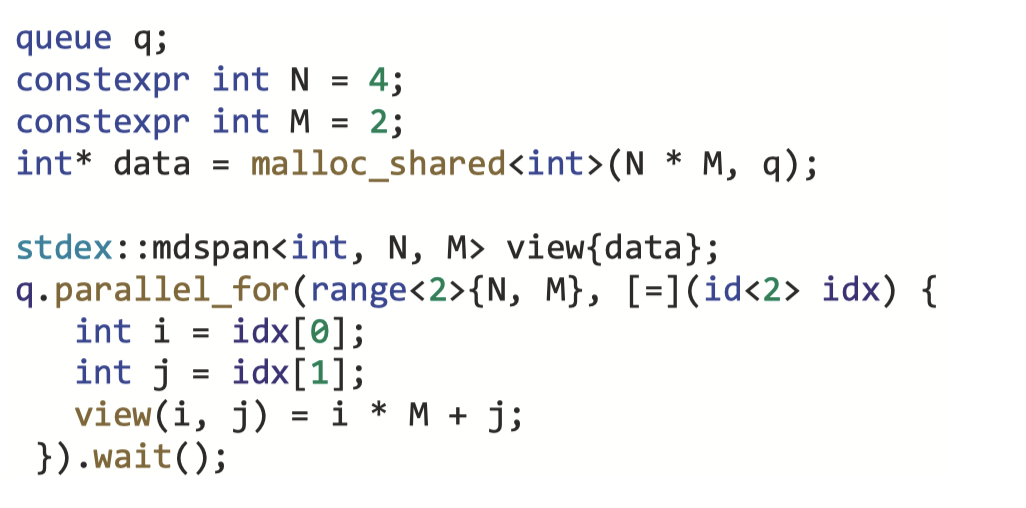
\includegraphics[width=0.9\textwidth]{figs/F22.1.png}
	\caption{\textit{统一内存简化了 CPU 代码(左)到 CUDA 代码(右)的移植。}}
\end{figure}

这样的好处之一就是减少了将 CPU 代码移植到 CUDA 所需的工作量。 在图 22.1 中,我们在左侧展示了一个简单的 CPU 代码示例。 
通过统一内存,只需进行两个简单的更改即可将代码移植到 CUDA。 
第一个更改是使用 cudaMallocManaged() 和 cudaFree() 代替 malloc() 和 free()。 
第二个更改是启动内核并执行设备同步,而不是调用 qsort() 函数。 
显然,人们仍然需要编写或访问并行 qsort 内核。 我们所展示的是对主机代码的更改是简单且易于维护的。

CUDA 6统一内存的性能受到Kepler和Maxwell GPU架构的硬件能力的限制。 
在任何网格启动之前,必须将 CPU 修改过的所有托管内存位置的内容刷新到 GPU 设备内存。 
CPU 和 GPU 无法同时访问托管内存分配,并且统一内存地址空间仅限于 GPU 物理内存的大小。 
这些限制是由于这些 GPU 架构缺乏支持主机和设备内存之间一致性的能力,并且数据迁移主要由软件执行。

2016 年,Pascal GPU 架构添加了一些功能,以进一步简化 CPU 和 GPU 之间的编程和内存共享,
并进一步减少使用 GPU 实现显着加速所需的工作量。 两个主要硬件功能实现了这些改进:支持大地址空间和页面错误处理能力。

Pascal GPU 架构将 GPU 寻址能力扩展到 49 位虚拟寻址。 
这个扩展足够大,可以覆盖现代 CPU 的 48 位虚拟地址空间以及 GPU 自己的内存。 
这使得统一内存程序能够将系统中所有 CPU 和 GPU 的完整地址空间作为单个虚拟地址空间进行访问,
而不受可拷贝到设备内存的数据量的限制。 因此,CPU 和 GPU 可以真正共享指针值,使 GPU 能够遍历主机内存中基于指针的数据结构。

Pascal GPU 架构中的内存页面错误处理支持是一项重要的新功能,可提供更无缝的统一内存功能。 
与系统范围的虚拟地址空间相结合,处理页面错误的能力使得 CUDA 系统软件无需在每次网格启动之前将所有托管内存内容同步(刷新)到 GPU。 
CUDA 运行时可以通过允许主机和设备在修改托管内存中的变量时使彼此的副本无效来实现一致性机制。 
可以通过使用页面映射和保护机制来完成失效。 启动网格时,CUDA 系统软件不再需要更新托管内存数据的所有 GPU 副本。 
如果网格访问设备内存中的副本已被主机失效的数据,GPU 将处理页面错误以使数据更新并恢复执行。

如果 GPU 上运行的网格访问未驻留在其设备内存中的页面,它也会发生页面错误,从而允许页面根据需要自动迁移到 GPU 内存。 
或者,如果预计仅偶尔访问数据,则可以将页面映射到 GPU 地址空间,以便通过系统互连进行访问(访问映射有时可能比迁移更快)。 
请注意,统一内存是系统范围内的:GPU(和 CPU)可以从 CPU 内存或系统中其他 GPU 的内存中故障和迁移内存页面。 
如果 CPU 函数解引用了指针并访问映射到 GPU 物理内存的变量,数据访问仍然会有效,但延迟可能会更长。 
这种功能允许 CUDA 程序更轻松地调用尚未移植到 GPU 的遗留库。 
在之前的 CUDA 内存架构中,开发人员必须手动将数据从设备内存传输到主机内存,以便使用遗留库函数在 CPU 上处理它们。

具有页面错误处理能力的统一内存可实现比零拷贝内存更通用的CPU/GPU交互机制。 它允许 GPU 遍历主机内存中的大型数据结构。 
从 Pascal 架构开始,GPU 设备可以遍历链表的数据结构,即使该数据结构不驻留在零拷贝内存中。 
这是因为主机代码和设备代码中使用相同的指针值来引用相同的变量。 
因此,设备可以遍历主机构建的链表数据结构的嵌入指针值,反之亦然。 
在某些应用领域,例如CAD,主机物理内存系统可能具有数百GB的容量。 
需要这些物理内存系统是因为应用程序要求整个数据集位于“核心”。 
由于能够直接访问非常大的 CPU 物理内存,GPU 可以加速这些应用程序。

\subsubsection{虚拟地址空间控制}
CUDA 11 引入了一组低级 API,为程序员提供了内存分配方面的更大灵活性。 
新的 API 允许使用 cuMemAddressReserve() 保留一定范围的虚拟地址空间。 
稍后,程序员可以使用 cuMemCreate() 在任何设备上分配物理内存,并使用 cuMemMap() 将其映射到保留范围中的任何位置。 
这些 API 允许跨多个设备构建数据结构的自定义布局。 例如,可以在多个设备上分配 3D 体积,同时使用单个指针来引用它。

\subsection{核函数执行控制}
\subsubsection{核函数内的函数调用}
早期的 CUDA 版本不允许在内核执行期间调用函数。 
虽然内核函数的源代码看起来可能有函数调用,但编译器必须能够将所有函数体内联到内核对象中,以便在运行时内核函数中不存在函数调用。 
尽管此模型对于许多应用程序的性能关键部分来说相当有效,但它不支持更复杂的应用程序中的常见软件工程实践。 
特别是,它不支持C++等面向对象语言中的系统调用、动态链接库调用、递归函数调用和虚函数。

后来的设备架构,例如开普勒,支持运行时内核函数中的函数调用。 CUDA 5 及更高版本支持此功能。 编译器不再需要内联函数体。 
它仍然可以作为性能优化来这样做。 此功能部分是通过缓存和对CUDA线程的快速并行的帧栈来实现的。 
它允许不同的作者编写不同的 CUDA 内核组件并将它们组装在一起,而无需大量的重新设计成本,从而使 CUDA 设备代码更加“可组合”。 
它还允许软件供应商发布没有源代码的设备库以保护知识产权。 然而,仍然存在一些限制。 
例如,对虚拟函数的支持仅限于设备代码构造的对象,并且不支持设备代码的动态库。

对运行时函数调用的支持还可以实现递归,并显着减轻程序员从传统的面向 CPU 的算法过渡到 GPU 调整的代码时的负担。 
在某些情况下,开发人员将能够将 CPU 代码“剪切并粘贴”到 CUDA 内核中,并获得性能合理的内核,尽管持续的性能调整仍然会带来好处。

有了函数调用支持,内核现在可以调用标准库函数,例如 printf() 和 malloc()。 
根据我们的经验,在内核中调用 printf() 的能力为调试和支持生产软件中的内核提供了微妙但重要的帮助。 
许多最终用户都是非技术人员,无法轻松接受培训来运行调试器,而调试器将为开发人员提供有关崩溃前发生的情况的更多详细信息。 
在内核中调用 printf() 的功能允许开发人员向应用程序添加一种模式来转储内部状态,以便最终用户可以提交有意义的错误报告。

CUDA 8 添加了对 C++11 的支持,以及另一种形式的函数调用:lambda。 
当与元编程技术结合使用时,设备 lambda 可以开发高性能可重用代码。 CUDA 还支持将 lambda 函数作为参数传递给 CUDA 内核。 
此功能可用于编写通用内核(例如排序内核),其中比较函数只是内核的输入参数。 
CUDA 还添加了对“扩展 lambda”的实验性支持,该支持通过“扩展 lambda”编译器标志启用。 
此功能允许程序员使用 \_\_host\_\_ \_\_device\_\_ 修饰符来注释 C++ lambda,从而进一步简化编写可重用代码的任务。

\subsubsection{核函数中的异常处理}
早期的 CUDA 系统不支持内核代码中的异常处理。 
虽然对于许多高性能应用程序的性能关键部分来说不是一个重大限制,但它通常会在生产质量应用程序中产生软件工程成本,
这些应用程序依赖异常来检测和处理罕见情况,而不执行代码来显式测试此类情况。

通过提供有限的异常处理支持,CUDA 调试器允许用户执行逐步执行、设置断点和/或运行内核,直到发生无效的内存访问。 
在每种情况下,用户都可以在执行暂停时检查内核的局部变量和全局变量的值。 
根据我们的经验,CUDA 调试器是一个非常有用的工具,可以检测越界内存访问和潜在的竞争条件。

\subsubsection{多个网格同时执行}
最早的 CUDA 系统在任何时间点只允许在每个 GPU 设备上执行一个网格。 
可以使用 CUDA 流提交多个网格来执行,但它们被缓冲在队列中,该队列在当前网格完成执行后释放下一个网格。 
Fermi GPU 架构及其后续产品允许同时执行同一应用程序的多个网格,
这减轻了应用程序开发人员将多个内核“批处理”为更大内核的压力,以便更充分地利用设备。 
此外,有时将工作划分为可以以不同优先级执行的块是有益的。

同时执行多个网格的好处的一个典型例子是并行集群应用程序,它将工作分为“本地”和“远程”分区,其中远程工作涉及与其他节点的交互,
并驻留在全局进展的关键路径上( 第 20 章,异构计算集群编程)。 
在以前的 CUDA 系统中,网格需要执行大量工作才能有效地利用设备,并且必须小心不要启动本地工作,以免阻止全局工作。 
这意味着要么在等待远程工作到达时充分利用设备,要么急切地开始本地工作以保持设备的生产力,
但代价是增加完成远程工作单元的延迟(Phillips 和 Stone,2009)。 
通过多个网格执行,应用程序可以使用更小的网格大小来启动工作,因此,当高优先级远程工作到达时,
它可以以低延迟开始运行,而不是陷入本地计算的大型网格后面。

\subsubsection{硬件队列和动态并行性}
在 Kepler 架构和 CUDA 5 中,通过添加多个硬件队列来扩展多网格启动设施,这允许更有效地调度来自多个流的多个网格的线程块。 
此外,第 21 章“CUDA 动态并行性”中介绍的 CUDA 动态并行性允许 GPU 工作创建:
GPU 网格可以以数据相关或计算负载相关的方式异步、动态地启动子网格。 
这减少了 CPU-GPU 交互和同步,因为 GPU 现在可以独立管理更复杂的工作负载。 CPU 又可以自由地执行其他有用的计算。

\subsubsection{可中断网格}
Fermi GPU 架构允许“取消”正在运行的网格,从而能够创建 CUDA 加速的应用程序,允许用户随时中止长时间运行的计算,
而无需程序员进行大量的设计工作。 这使得用户级任务调度系统的实现能够更好地执行计算系统的 GPU 节点之间的负载平衡,
并允许更优雅地处理一个 GPU 负载较重且可能比其他 GPU 运行得更慢的情况(Stone 和 Hwu) ,2009)。

\subsubsection{合作核函数}
处理不规则数据的 GPU 内核经常会遇到负载不平衡的问题。 CUDA 11 引入了协作内核来缓解这个问题。 
协作内核最多可以执行完全填满 GPU 的最大数量的线程块,并且 CUDA 运行时保证所有线程块将同时执行。 
这种并发保证使线程块能够安全地协作,而不会在可用于保护共享数据结构(例如工作队列)的共享互斥机制(例如互斥体)上出现死锁。 
协作内核需要特殊的 API cudaLaunchCooperativeKernel(),并提供设备 API 来识别和分区线程组。 
协作内核不限于单个设备,而是可以使用 cudaLaunchCooperativeKernelMultiDevice() 调用在多个设备中运行。

\subsection{内存带宽和计算吞吐量}
\subsubsection{双精度速度}
早期的设备执行双精度浮点运算,与单精度相比,速度显着降低(大约慢八倍)。 
费米及其后继者的浮点运算单元得到了显着增强,能够以大约单精度一半的速度执行双精度运算。 
大量使用双精度浮点运算的应用程序受益匪浅。

在实践中,最显着的好处是由将基于 CPU 的数值应用程序移植到 GPU 的开发人员获得的。 
随着双精度速度的提高,他们几乎没有动力花精力去评估他们的应用程序或部分应用程序是否适合单精度。 
这显着降低了将 CPU 应用程序移植到 GPU 的开发成本,并解决了 HPC 社区早期对 GPU 的主要批评。

一些在较小输入数据类型(8 位、16 位或单精度浮点)上运行的应用程序继续受益于使用单精度算术,
因为与 64 位数据相比,使用 32 位数据减少了带宽 。 
医学成像、遥感、射电天文学、地震分析和其他自然数据等应用通常属于这一类别。 
Pascal GPU架构引入了对16位半精度数计算的新硬件支持,以进一步提高数据适合半精度表示的应用程序的性能和能效。 
例如,基于Ampere架构的A100,使用张量核的16位半精度算术吞吐量为156 TFLOPS,相比其19.5 TFLOPS单精度吞吐量有了巨大的提升。

\subsubsection{更高的控制流效率}
从 Fermi GPU 架构开始,CUDA 系统采用了通用编译器驱动的预测技术(Mahlke 等人,1995,
该技术可以比以前的 CUDA 系统更有效地处理控制流。 虽然该技术在 VLIW 系统中取得了一定的成功,
但它在 GPU warp 式 SIMD 执行系统中提供了更显着的速度改进。 
此功能扩大了可以利用 GPU 的应用程序范围。 特别是,对于数据驱动的应用程序(例如光线追踪、量子化学可视化和元胞自动机模拟),可以实现主要的性能优势。

\subsubsection{可配置的缓存和暂存器}
早期 CUDA 系统中的共享内存充当程序员管理的暂存器内存,并提高了关键数据结构具有本地化和可预测访问模式的应用程序的速度。 
从Fermi GPU架构开始,共享内存被增强为更大的芯片上内存,可以配置为部分高速缓存和部分共享内存,
这使得覆盖可预测和不太可预测的访问模式都可以从芯片上受益 记忆。 这种可配置性允许程序员根据最适合其应用程序的方式分配资源。

直接从 CPU 代码移植的早期设计阶段的应用程序将大大受益于作为芯片上存储器的主要部分的缓存。 
当开发人员将 CPU 应用程序移植到 GPU 时,这会提高“轻松性能”的级别,从而进一步简化性能调整过程。

现有的 CUDA 应用程序和具有可预测访问模式的应用程序能够增加对快速共享内存的使用,同时保留与上一代设备相同的设备“占用率”。 
对于性能或功能受到共享内存大小限制的 CUDA 应用程序来说,大小的增加将是一个可喜的改进。 
例如,在模板计算(第8章“模板”和第20章“异构计算集群编程”)中,
例如计算流体动力学的有限差分方法,增加的共享内存容量提高了内存带宽效率和应用程序的性能。

\subsubsection{增强的原子操作}
Fermi GPU架构中的原子操作比以前的CUDA系统中的原子操作要快得多,开普勒中的原子操作甚至更快。 
此外,开普勒原子操作更加通用。 Maxwell GPU 架构中共享内存变量的原子操作的吞吐量得到了进一步增强。 
原子操作经常用于随机分散计算模式,例如直方图(第 9 章,并行直方图:原子操作和私有化简介)。 
更快的原子操作减少了对算法转换的需求,例如前缀和(第 11 章,前缀和(扫描):并行算法工作效率简介)
(Sengupta 等人,2007)和排序(第 13 章,排序)(Satish) et al., 2009)用于实现这种随机散射计算。 
这些转换往往会增加内核调用的数量以及执行目标计算所需的操作总数。 
更快的原子操作还可以减少主机 CPU 参与集体操作或多个线程块更新共享数据结构的算法的需要,
从而减少 CPU 和 GPU 之间的数据传输压力。

\subsubsection{增强的全局内存访问}
Fermi 和 Kepler 中的随机内存访问速度比早期 GPU 架构快得多。 程序员可以不太关心内存合并。 
这使得更多的CPU算法可以直接在GPU中用作可接受的基础,进一步平滑了访问多种数据结构的应用程序的移植路径,
例如光线追踪,以及其他严重面向对象且可能很困难的应用程序 转换为完美tile的数组。

Pascal GPU 架构采用了 HBM2(高带宽内存版本 2)3D 堆叠 DRAM 内存,
可提供高达上一代 NVIDIA Maxwell 架构 GPU 内存带宽的 $3 \times$ 倍。 
Pascal 也是第一个支持 NVLink 处理器互连的架构,
这使得 Tesla P100 的 GPU-GPU 和 GPU-CPU 通信性能高达 PCI Express 3.0 的 $5 \times$ 。 
这种互连极大地提高了节点内多 GPU 计算的可扩展性以及 GPU 和支持 NVLink 的 CPU 之间的数据共享效率。

\subsection{编程环境}
\subsubsection{统一设备内存空间}
在早期的 CUDA 设备中,共享内存、本地内存和全局内存形成了自己独立的地址空间。 
开发人员可以使用指向全局内存的指针,但不能使用其他内存。 
从 2009 年推出的 Fermi 架构开始,这些存储器成为统一地址空间的一部分。 
这种统一的地址空间使一组加载/存储指令和指针地址能够访问任何 GPU 内存空间(全局、本地或共享内存),
而不是为每个内存空间使用不同的指令和指针。 
这使得更容易抽象出包含特定操作数的内存,允许程序员仅在分配期间处理此问题,
并使将 CUDA 数据对象传递到其他过程和函数中更简单,无论它们来自哪个内存区域。

这使得 CUDA 代码模块更加“可组合”。 也就是说,CUDA 设备函数可以接受可能指向这些存储器中的任何一个的指针。 
例如,如果没有统一的 GPU 地址空间,设备函数需要为其参数之一可以驻留的每种类型的内存提供一种实现。 
统一的 GPU 地址空间允许以相同的方式访问所有主要类型的 GPU 内存中的变量,
从而允许一个设备函数接受可以驻留在不同类型的 GPU 内存中的参数。 
如果函数参数指针指向共享内存位置,则代码运行速度会更快;如果指向全局内存位置,则代码运行速度会更慢。 
程序员仍然可以执行手动数据放置和传输作为性能优化。 此功能显着降低了构建生产质量 CUDA 库的成本。 
这还启用了完整的 C 和 C++ 指针支持,这在当时是一个重大进步。

未来的 CUDA 编译器将增强对 C++ 模板和内核函数中的虚拟函数调用的支持。 
尽管硬件增强(例如运行时函数调用能力)已经到位,但编译器中增强的 C++ 语言支持仍需要更多时间。 
通过这些增强功能,未来的 CUDA 编译器将支持大多数主流 C++ 功能。 
例如,已经支持在内核函数中使用 new、delete、构造函数和析构函数等 C++ 功能。

新的和改进的编程接口继续提高异构并行程序员的生产力。 
OpenACC 允许开发人员使用编译器指令注释他们的顺序循环,以使编译器能够生成 CUDA 内核。 
人们可以使用并行泛型函数、类和迭代器的 Thrust 库来描述它们的计算,并让底层机制生成和配置实现计算的内核。 
CUDA FORTRAN 允许 FORTRAN 程序员用他们熟悉的语言开发 CUDA 内核。 
特别是,CUDA FORTRAN 为多维数组索引提供了强大的支持。 
C++AMP 允许开发人员将其内核描述为对逻辑数据结构(例如 C++ 应用程序中的多维数组)进行操作的并行循环。 
我们完全期望新的创新将不断出现,以进一步提高开发人员在这个令人兴奋的领域的生产力。

\subsubsection{通过关键路径分析进行分析}
在 CPU 和 GPU 上进行大量计算的异构应用程序中,找到花费优化工作的最佳位置可能是一个挑战。 
理想情况下,在优化代码时,人们希望以应用程序中能够以最少的努力提供最高加速的位置为目标。 
为此,CUDA 7.5 引入了 PC 采样,提供指令级分析,以便用户可以查明在其应用程序中占用最多时间的特定代码行。

\begin{figure}[H]
	\centering
	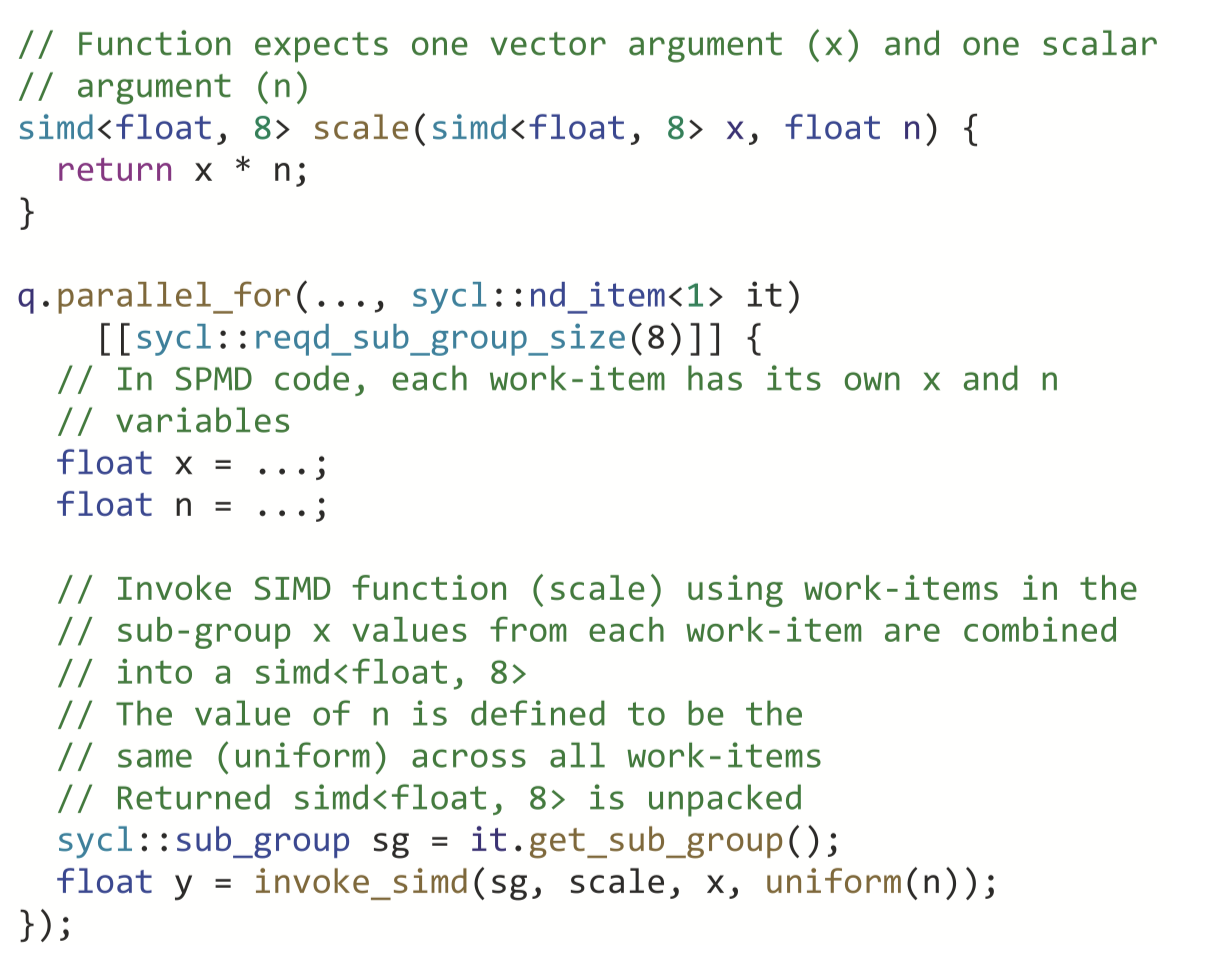
\includegraphics[width=0.9\textwidth]{figs/F22.2.png}
	\caption{\textit{关键路径分析对于识别要优化的关键内核的重要性。}}
\end{figure}

然而,此类分析器的用户面临的一个挑战是应用程序中运行时间最长的内核并不总是最关键的优化目标。 
如图 22.2 所示,内核 X 是运行时间较长的内核。 然而,它的执行时间与CPU执行活动A完全重叠。
内核X的执行时间的任何进一步改进而不同时改进A的执行时间不太可能提高应用程序性能。 
虽然内核Y的执行时间不如内核X长,但它处于应用程序执行的关键路径上。 
CPU在等待Kernel Y完成时处于空闲状态。加速Kernel Y会减少CPU等待的时间,因此它是最好的优化目标。

\begin{figure}[H]
	\centering
	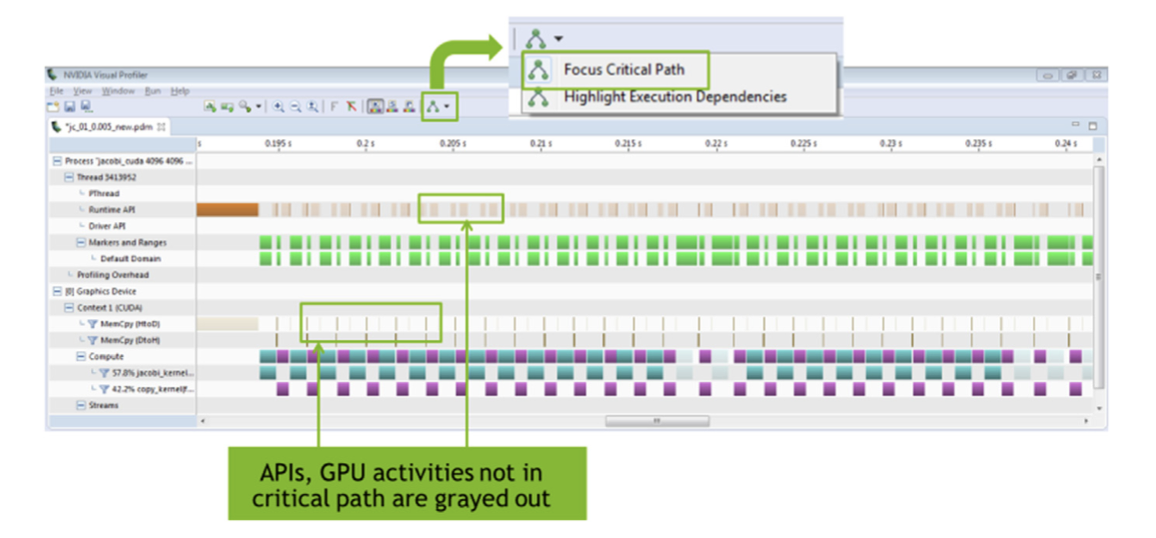
\includegraphics[width=0.9\textwidth]{figs/F22.3.png}
	\caption{\textit{CUDA 8 Visual Profiler 中的应用程序关键路径分析。}}
\end{figure}

2016 年,CUDA 8 中的 Visual Profiler 提供了 GPU 内核和 CPU CUDA API 调用之间的关键路径分析,
从而能够更精确地定位优化工作。 图 22.3 显示了 CUDA 8 Visual Profiler 中的关键路径分析。 
不在关键路径上的 GPU 内核、副本和 API 调用呈灰色显示。 仅应用程序执行的关键路径上的活动以颜色突出显示。 
这使用户可以轻松识别内核和其他活动,以针对用户的优化工作。

\subsection{未来展望}
CUDA 的发展不断增强其对开发人员生产力和现代软件工程实践的支持。 
借助新功能和编程语言支持,能够以最低开发成本获得合理性能的应用程序范围将显着扩大。 
与以前的 CUDA 系统相比,开发人员体验到了应用程序开发、移植和维护成本的降低。 
使用 Thrust 和自动生成 CUDA 代码的类似高级工具开发的现有应用程序也可能会立即提高性能。 
虽然内存架构、内核执行控制和计算核心性能方面的硬件增强的好处将在相关的 SDK 版本中显现出来,
但这些增强的真正潜力可能需要数年时间才能在 SDK 和运行时中得到充分利用。 
我们预测,未来几年,业界和学术界在 GPU 计算的编程工具和运行时环境方面将迎来激动人心的创新时刻。